\begin{figure}[H]
    \centering
    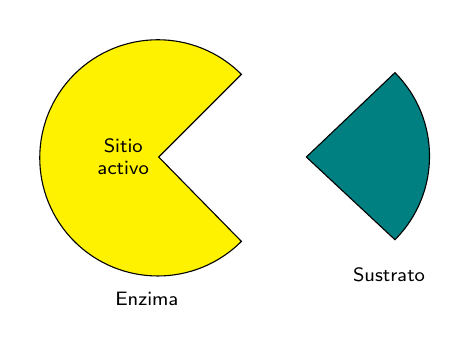
\begin{tikzpicture}[scale=1.5]
        \draw[fill=yellow] (0,0) -- (0.7,0.7) arc (45:315:1) -- cycle;
        \draw[fill=teal] (1.25,0) --++ (0.75,-0.7) arc (-45:45:1) -- cycle;
        \node[font=\scriptsize\sffamily] at (-0.1,-1.2) {Enzima};
        \node[font=\scriptsize\sffamily] at (1.95,-1) {Sustrato};
        \node[align=center, font=\scriptsize\sffamily] at (-0.3,0) {Sitio\\activo};
    \end{tikzpicture}
    \rule{\linewidth}{0.2pt}
    \caption{Estructura de una enzima}
    \label{fig:estructura_de_una_enzima}
\end{figure}